\chapter{Calcolo di autovalori e autovettori}
	
	\noindent Il calcolo degli autovalori di una data matrice quadrata \(A\) di ordine \(n\) consiste nel trovare gli \(n\) numeri \(\lambda_1, \dots, \lambda_n\) tali che esista \(x \ne \vec{0}\) tale che \(A x = \lambda_i x\) per un certo \(i \in \Set{1, \dots, n}\).
	
	È noto che gli autovalori di \(A\) sono anche gli zeri del polinomio caratteristico \(p_A (X) = \det (A - X \uno_n)\), perciò sono \(n\) numeri complessi, se contati con molteplicità.
	
	Nelle applicazioni talvolta si richiede di calcolare tutti gli autovalori di \(A\), talvolta solo alcuni -- ad esempio solo quelli di massimo modulo, in modo da determinare il raggio spettrale di \(A\).
	
\section{Teoremi di Gerschgorin}
	
	\begin{teorema}[Gerschgorin \textsc{i}]\label{th:gerschgorin-1}
		Data una matrice quadrata \(A\) di ordine \(n\) e di autovalori \(\lambda_1, \dots, \lambda_n\) e definiti per ogni \(i \in \Set{1, \dots, n}\)
		\begin{equation*}
			K_i = \Set{z \in \C : \abs{z - a_{i, i}} \le \sum_{\substack{j = 1 \\ j \ne i}}^n \abs{a_{i, j}}}
		\end{equation*}
		si verifica
		\begin{equation}\label{eq:gerschgorin-1}
			\Set{\lambda_1, \dots, \lambda_n} \subseteq \bigcup_{i = 1}^n K_i
		\end{equation}
	\end{teorema}

	\begin{esempio}\label{eg:gersch-1}
		Consideriamo la matrice
		\begin{equation*}
			A =
			\begin{pmatrix}
				15 & -2 & 2  \\
				1  & 10 & -3 \\
				-2 & 1  & 0
			\end{pmatrix}
		\end{equation*}
		I suoi cerchi di Gerschgorin sono
		\begin{align*}
			K_1 &= \Set{z \in \C : \abs{z - 15} \le 4} \\
			K_2 &= \Set{z \in \C : \abs{z - 10} \le 4} \\
			K_3 &= \Set{z \in \C : \abs{z} \le 3}
		\end{align*}
		Per il Teorema~\ref{th:gerschgorin-1}, gli autovalori di \(A\) appartengono all'unione di questi tre cerchi, come si può vedere nella Figura~\ref{fig:gersch-1}.
		
		\begin{figure}[tpb]
			\centering
			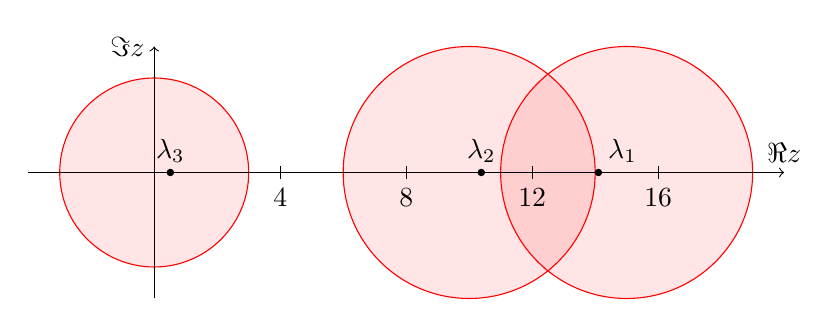
\begin{tikzpicture}[scale=0.4]
				\filldraw[color = red, fill opacity = 0.1] (15,0) circle[radius=4];
				\filldraw[color = red, fill opacity = 0.1] (10,0) circle[radius=4];
				\filldraw[color = red, fill opacity = 0.1] (0,0) circle[radius=3];
				\filldraw (14.1026,0) circle[radius=0.1] node [above right] {\(\lambda_1\)};
				\filldraw (10.3854,0) circle[radius=0.1] node [above] {\(\lambda_2\)};
				\filldraw (0.512085,0) circle[radius=0.1] node [above] {\(\lambda_3\)};
				\draw[->] (-4,0) -- (20,0) node [above] {\(\Re z\)};
				\draw[->] (0,-4) -- (0,4) node [left] {\(\Im z\)};
				\foreach \i in {4, 8, 12, 16} {
					\draw (\i, 0.2) -- (\i, -0.2) node [below] {\i};	
				}
			\end{tikzpicture}
			
			\caption{Rappresentazione dei cerchi di Gerschgorin e degli autovalori relativi alla matrice \(A\) dell'Esempio~\ref{eg:gersch-1}.}\label{fig:gersch-1}
		\end{figure}
	\end{esempio}

	\begin{teorema}[Gerschgorin \textsc{ii}]\label{th:gerschgorin-2}
		Se l'unione \(M_1\) di \(k\) cerchi di Gerschgorin è disgiunta dall'unione \(M_2\) dei rimanenti \(n - k\) cerchi, allora \(M_1\) contiene esattamente \(k\) autovalori di \(A\) contati con molteplicità e \(M_2\) contiene esattamente \(n - k\) autovalori di \(A\) contati con molteplicità.
	\end{teorema}

	Guardando la Figura~\ref{fig:gersch-1}, è evidente che la matrice \(A\) dell'Esempio~\ref{eg:gersch-1} abbia un solo autovalore in \(K_1\) e due autovalori in \(K_2 \cup K_3\).
	
	\begin{definizione}
		Una matrice quadrata \(A\) di ordine \(n \ge 2\) si dice \emph{riducibile} se esistono una matrice di permutazione \(P\) e un intero \(k \in \Set{1, \dots, n - 1}\) tali che
		\begin{equation}
			P \! A \tra{P} =
			\begin{pmatrix}
				A_{1, 1} & A_{1, 2} \\
				\zero    & A_{2, 2}
			\end{pmatrix}
		\end{equation}
		con \(A_{1, 1} \in M_k (\C)\) e \(A_{2, 2} \in M_{n - k} (\C)\).
		
		Una matrice quadrata si dice \emph{irriducibile} se non è riducibile.
	\end{definizione}

	Per verificare che una matrice sia irriducibile, ricordiamo che una matrice quadrata \(A\) è irriducibile se e solo se il suo grafo orientato associato è fortemente connesso, ovvero se e solo se per ogni coppia \((i, j)\) esiste un cammino da \(i\) verso \(j\).\footnote{A partire da una matrice quadrata \(A\) di ordine \(n\) se ne costruisce il grafo orientato associato ponendo \(1, \dots, n\) come nodi e tracciando il lato \((i, j)\) se e solo se \(a_{i, j} \ne 0\).} Nella Figura~\ref{fig:grafo-gersch-1} è rappresentato il grafo orientato associato alla matrice \(A\) dell'Esempio~\ref{eg:gersch-1}: in base ad esso, si può affermare che \(A\) è irriducibile.
	
	\begin{figure}[tpb]
		\centering
		
		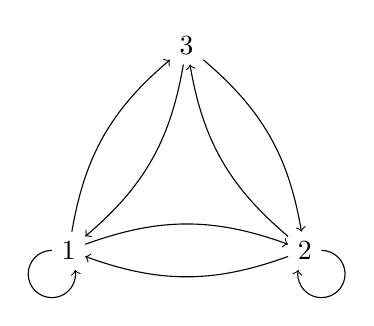
\begin{tikzpicture}[scale = 3]
			\node (a) at (0,0) {1};
			\node (b) at (1,0) {2};
			\node (c) at (0.5,0.866) {3};
			
			\draw[->] (a) to[bend left = 20] (b);
			\draw[->] (a) to[bend left = 20] (c);
			\draw[->] (b) to[bend left = 20] (a);
			\draw[->] (b) to[bend left = 20] (c);
			\draw[->] (c) to[bend left = 20] (a);
			\draw[->] (c) to[bend left = 20] (b);
			
			\draw[->] (a.west) arc[start angle = 90, end angle = 370, radius = 1mm];
			\draw[->] (b.east) arc[start angle = 90, end angle = -190, radius = 1mm];
		\end{tikzpicture}
	
		\caption{Grafo orientato associato alla matrice \(A\) dell'Esempio~\ref{eg:gersch-1}.}\label{fig:grafo-gersch-1}
	\end{figure}

	\begin{teorema}[Gerschgorin \textsc{iii}]\label{th:gerschgorin-3}
		Se una matrice quadrata \(A\) di ordine \(n\) è irriducibile e un suo autovalore \(\lambda\) appartiene alla frontiera dell'unione dei cerchi di Gerschgorin di \(A\), allora \(\lambda\) appartiene alla frontiera di ogni cerchio di Gerschgorin di \(A\).
	\end{teorema}

	\begin{esempio}\label{eg:gersch-2}
		Consideriamo la matrice
		\begin{equation*}
			B =
			\begin{pmatrix}
				2  & -1 & 0  & 0  \\
				-1 & 2  & -1 & 0  \\
				0  & -1 & 2  & -1 \\
				0  & 0  & -1 & 2
			\end{pmatrix}
		\end{equation*}
		Essa è irriducibile, come mostra il suo grafo orientato nella Figura~\ref{fig:grafo-gersch-2}. Per il Teorema~\ref{th:gerschgorin-1} tutti gli autovalori di \(B\) appartengono alla palla chiusa di centro \(2\) e raggio \(2\), ma non possono appartenere contemporaneamente alle frontiere di tutti i cerchi di Gerschgorin; per questo motivo, dal Teorema~\ref{th:gerschgorin-3} segue che \(B\) è non singolare.
		
		\begin{figure}[tpb]
			\centering
			
			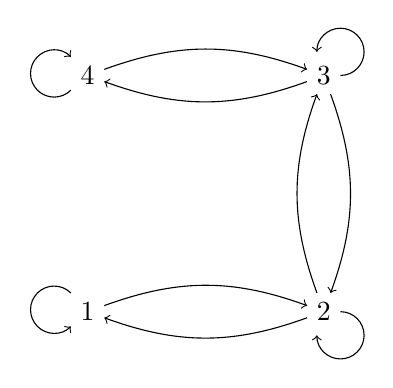
\begin{tikzpicture}[scale = 3]
				\node (a) at (0,0) {1};
				\node (b) at (1,0) {2};
				\node (c) at (1,1) {3};
				\node (d) at (0,1) {4};
				
				\draw[->] (a) to[bend left = 20] (b);
				\draw[->] (b) to[bend left = 20] (a);
				\draw[->] (b) to[bend left = 20] (c);
				\draw[->] (c) to[bend left = 20] (b);
				\draw[->] (c) to[bend left = 20] (d);
				\draw[->] (d) to[bend left = 20] (c);
				
				\draw[->] (a.north west) arc[start angle = 45, end angle = 315, radius = 1mm];
				\draw[<-] (d.north west) arc[start angle = 45, end angle = 315, radius = 1mm];
				\draw[->] (b.east) arc[start angle = 90, end angle = -180, radius = 1mm];
				\draw[->] (c.east) arc[start angle = -90, end angle = 180, radius = 1mm];
			\end{tikzpicture}
			
			\caption{Grafo orientato associato alla matrice \(B\) dell'Esempio~\ref{eg:gersch-2}.}\label{fig:grafo-gersch-2}
		\end{figure}
	\end{esempio}

	\begin{osservazione}
		Poiché \(\tra{A}\) ha gli stessi autovalori di \(A\), è possibile raffinare il criterio dei cerchi di Gerschgorin affermando che gli autovalori di \(A\) appartengono all'intersezione tra l'unione dei cerchi di Gerschgorin di \(A\) e l'unione dei cerchi di Gerschgorin di \(\tra{A}\).
	\end{osservazione}

\section{Metodo delle potenze}
	
	\noindent Il metodo delle potenze si usa per calcolare l'autovalore di massimo modulo di una matrice quadrata. Nel nostro caso supporremo sempre che la matrice \(A\) sia quadrata, di ordine \(n\), diagonalizzabile e tale che i suoi autovalori \(\lambda_1, \dots, \lambda_n\) verifichino\(\abs{\lambda_1} > \abs{\lambda_2} \ge \dots \ge \abs{\lambda_n}\).
	
	Ricordiamo che una matrice quadrata \(A\) di ordine \(n\) è diagonalizzabile se e solo se ammette \(n\) autovettori linearmente indipendenti. Ricordiamo anche che, se \(A\) ammette \(n\) autovalori distinti, allora è diagonalizzabile; se \(A\) è simmetrica o hermitiana, allora è diagonalizzabile.
	
	\begin{teorema}\label{th:metodo-potenze-converge}
		Data una matrice \(A \in M_n (\C)\) diagonalizzabile e con autovalori \(\lambda_1, \dots, \lambda_n\) tali che \(\abs{\lambda_1} > \abs{\lambda_2} \ge \dots \ge \abs{\lambda_n}\) e scelti \(u_1, \dots, u_n \in \C^n \setminus \Set{\vec{0}}\) tali che \(A u_k = \lambda_k u_k\) per ogni \(k \in \Set{1, \dots, n}\), se il vettore \(y_0 = \sum_{k = 1}^n \alpha_k u_k\) verifica \(\alpha_1 \ne 0\), allora la successione \((y_s)_{s \in \N}\) definita da
		\begin{equation}
			y_{s + 1} = A y_s
		\end{equation}
		per ogni \(s \in \N\) converge per direzione alla direzione di \(u_1\) e il \emph{quoziente di Rayleigh}
		\begin{equation}
			\rayleigh (y_s, A) = \frac{(A y_s, y_s)}{(y_s, y_s)}
		\end{equation}
		converge a \(\lambda_1\).
	\end{teorema}

	\begin{proof}
		Poiché \(A\) è diagonalizzabile, i vettori \(u_1, \dots, u_n\) esistono certamente e, essendo \(n\), formano una base di \(\C^n\). Visto che gli \(u_k\) sono autovettori relativi agli autovalori \(\lambda_k\), si ha
		\begin{align*}
			y_1 &= A y_0 = A \qty(\sum_{k = 1}^n \alpha_k u_k) = \sum_{k = 1}^n \alpha_k A u_k = \sum_{k = 1}^n \alpha_k \lambda_k u_k \\
			y_{s + 1} &= A y_s = A \qty(\sum_{k = 1}^n \alpha_k \lambda_k^s u_k) = \sum_{k = 1}^n \alpha_k \lambda_k^s A u_k = \sum_{k = 1}^n \alpha_k \lambda_k^{s + 1} u_k
		\end{align*}
		Da ciò segue che
		\begin{equation*}
			\frac{y_{s + 1}}{\lambda_1^{s + 1}} = \sum_{k = 1}^n \alpha_k \frac{\lambda_k^{s + 1}}{\lambda_1^{s + 1}} u_k = \alpha_1 u_1 + \sum_{k = 2}^n \alpha_k \qty(\frac{\lambda_k}{\lambda_1})^{s + 1} u_k
		\end{equation*}
		e, dato che \((\lambda_k / \lambda_1)^{s + 1} \xrightarrow{s \to \infty} 0\), si è provato che la direzione di \(y_s / \lambda_1^s\) converge a quella di \(u_1\).
		
		Dalla continuità del prodotto scalare usuale e di \(A\) segue che
		\begin{equation*}
			\begin{split}
				\lim_{s \to \infty} \rayleigh (y_s, A) &= \lim_{s \to \infty} \frac{(A y_s, y_s)}{(y_s, y_s)} = \lim_{s \to \infty} \frac{\qty(A \frac{y_s}{\lambda_1^s}, \frac{y_s}{\lambda_1^s})}{\qty(\frac{y_s}{\lambda_1^s}, \frac{y_s}{\lambda_1^s})} \\
				&= \frac{\qty(\lim_{s \to \infty} A \frac{y_s}{\lambda_1^s}, \lim_{s \to \infty} \frac{y_s}{\lambda_1^s})}{\qty(\lim_{s \to \infty} \frac{y_s}{\lambda_1^s}, \lim_{s \to \infty} \frac{y_s}{\lambda_1^s})} \\
				&= \frac{\qty(\alpha_1 A u_1, \alpha_1 u_1)}{\qty(\alpha_1 u_1, \alpha_1 u_1)} = \frac{(A u_1, u_1)}{(u_1, u_1)} = \frac{\cancel{(u_1, u_1)}}{\cancel{(u_1, u_1)}} \lambda_1 \\
				&= \lambda_1 \qedhere
			\end{split}
		\end{equation*}
	\end{proof}

	\begin{osservazione}
		Il Teorema~\ref{th:metodo-potenze-converge} mostra che il metodo delle potenze converge anche nel caso in cui \(\lambda_1 = \dots = \lambda_r\) per \(r > 1\), ma non quando esistono piú autovalori distinti di modulo massimo.
	\end{osservazione}

	\begin{osservazione}
		Per ovviare a problemi di \inglese{underflow} e \inglese{overflow}, in aritmetica di macchina si preferisce normalizzare ad ogni iterazione il vettore \(y_k\) ottenuto dal metodo delle potenze. Scelto, dunque, un vettore unitario \(t_0 = \sum_{k = 1}^n \alpha_k u_k\) con \(\alpha_1 \ne 0\), il metodo estrae le successioni \((t_k)_{k \in \N}\) e \((I_k)_{k \in \N}\) come segue:
		\begin{align}
			\gamma_k &= A t_{k - 1} &
			t_k &= \frac{\gamma_k}{\norm{\gamma_k}_2} &
			I_k &= \rayleigh (t_k, A)
		\end{align}
	\end{osservazione}

\section{Metodo delle potenze inverse}
	
	\noindent Il \emph{metodo delle potenze inverse} è una variante del metodo delle potenze usata per calcolare l'autovettore piú piccolo in modulo di una matrice quadrata \(A\) di ordine \(n\) e diagonalizzabile. Nel nostro caso, supporremo che gli autovalori \(\lambda_1, \dots, \lambda_n\) verifichino \(\abs{\lambda_1} \ge \dots \ge \abs{\lambda_{n - 1}} > \abs{\lambda_n} > 0\); in questo modo, possiamo ottenere \(\lambda_n\) applicando il metodo delle potenze alla matrice \(A^{-1}\).
	
	\begin{lemma}\label{lem:autovalori-inversa}
		Se una matrice quadrata \(A\) ha autovalori \(\lambda_1, \dots, \lambda_n\) tali che \(\abs{\lambda_1} \ge \dots \ge \abs{\lambda_n} > 0\) ed esistono \(u_1, \dots, u_n \in \C^n \setminus \Set{\vec{0}}\) tali che \(A u_k = \lambda_k u_k\) per ogni \(k \in \Set{1, \dots, n}\), allora \(A^{-1}\) ha come autovalori \(\xi_1, \dots, \xi_n\) che verificano \(\abs{\xi_1} \ge \dots \ge \abs{\xi_n} > 0\) e \(\xi_k = 1 / \lambda_{n - k + 1}\) per ogni \(k \in \Set{1, \dots, n}\) e i vettori \(v_k = u_{n - k + 1}\) sono tali che \(A^{-1} v_k = \xi_k v_k\).
	\end{lemma}

	Applicando il metodo delle potenze alla matrice \(A^{-1}\), supposto che \(A\) sia diagonalizzabile e che i suoi autovettori verifichino \(\abs{\lambda_1} \ge \dots \ge \abs{\lambda_{n - 1}} > \abs{\lambda_n} > 0\), si parte da un vettore unitario \(t_0 = \sum_{k = 0}^n \alpha_k u_k\) con \(\alpha_1 \ne 0\) e si ottiene la successione \((t_s)_{s \in \N}\) definita da
	\begin{align}
		\gamma_s &= A^{-1} t_{s - 1} &
		t_s &= \frac{\gamma_s}{\norm{\gamma_s}_2}
	\end{align}
	e convergente per direzione alla direzione di \(v_1 = u_n\). La successione dei quozienti di Rayleigh, invece, verifica
	\begin{equation*}
		\rayleigh (t_s, A^{-1}) = \frac{\qty(A^{-1} t_s, t_s)}{(t_s, t_s)} = (t_s, \gamma_{s + 1}) \to \xi_1 = \frac{1}{\lambda_n}
	\end{equation*}
	ovvero \(\rayleigh (t_s, A) \to \lambda_n\).
	
	In generale, fissato \(\mu \in \C\), è possibile calcolare con un algoritmo simile l'autovalore \(\lambda\) di \(A\) piú vicino a \(\mu\), qualora sia unico. Osservando, infatti, che
	\begin{equation*}
		A u = \lambda u \iff (A - \mu \uno_n) u = \lambda u - \mu u = \underbrace{(\lambda - \mu)}_{\sigma} u
	\end{equation*}
	segue che, se \(\sigma\) è un autovalore di minimo modulo di \(A - \mu \uno_n\), allora \(\lambda = \sigma + \mu\) è uno degli autovalori di \(A\) di minima distanza da \(\mu\) e che, se \(u\) è autovettore per \(\sigma\) relativamente ad \(A - \mu \uno_n\), allora lo è anche per \(\lambda\) relativamente ad \(A\). Qualora sia possibile applicare il metodo delle potenze inverse alla matrice \(A - \mu \uno_n\), scelto un vettore unitario \(t_0\), si definisce il metodo delle potenze inverse con \inglese{shift} con
	\begin{align}
		(A - \mu \uno_n) \gamma_k &= t_{k - 1} &
		t_k &= \frac{\gamma_k}{\norm{\gamma_k}_2} &
		\sigma_k &= \her{t_k} A t_k
	\end{align}

\section[Metodo \textsc{qr}]{Metodo QR}
	
	\noindent Il metodo \textsc{qr} si usa per calcolare efficientemente tutti gli autovalori di una matrice quadrata \(A\).
	
	\begin{teorema}[Fattorizzazione \textsc{qr}]\label{th:fattoriz-qr}
		Se \(A\) è una matrice quadrata di ordine \(n\), allora esistono una matrice \(Q\) unitaria e una matrice \(R\) triangolare superiore tali che \(A = Q R\).
	\end{teorema}
	
	Il Teorema~\ref{th:fattoriz-qr} garantisce l'esistenza di una fattorizzazione \textsc{qr} per \emph{qualunque} matrice quadrata. In generale, però, tale fattorizzazione non è unica, bensí determinata a meno di una matrice di fase. Qualora, invece, \(A\) sia non singolare, la fattorizzazione è unica se si richiede che i coefficienti diagonali di \(R\) siano positivi.
	
	Ricordiamo che, se \(H\) è simile a \(K\), cioè se esiste \(S\) invertibile tale che \(H = S^{-1} K S\), allora \(H\) e \(K\) hanno gli stessi autovalori -- e tale relazione è transitiva.
	
	\begin{lemma}\label{lem:a0-a1-simili}
		Data la fattorizzazione \textsc{qr} \(A_0 = Q_0 R_0\) e la matrice \(A_1 = R_0 Q_0\), le matrici \(A_0\) e \(A_1\) sono simili.
	\end{lemma}
	
	\begin{proof}
		È sufficiente notare che
		\begin{equation*}
			Q_0 A_1 \tra{Q_0} = Q_0 R_0 Q_0 \tra{Q_0} = A_0 \qedhere
		\end{equation*}
	\end{proof}

	Sulla base del Lemma~\ref{lem:a0-a1-simili} definiamo il metodo \textsc{qr}. Posto \(A_0 = A\), si calcolano le iterate \(A_k\) secondo la regola
	\begin{equation}
		A_k = Q_k R_k \implies A_{k + 1} = R_k Q_k
	\end{equation}
	ove ad ogni iterazione si calcola la fattorizzazione \textsc{qr} della matrice \(A_k\). Tutte le matrici \(A_k\) sono simili alla matrice \(A\) e, quindi, hanno gli stessi autovalori di \(A\).
	
	\begin{teorema}[Convergenza del metodo \textsc{qr}]\label{th:metodo-qr-converge}
		Se una matrice \(A \in M_n (\R)\) ha autovalori tutti distinti in modulo, ovvero \(\abs{\lambda_1} > \dots > \abs{\lambda_n}\), allora il metodo \textsc{qr} converge a una matrice triangolare superiore \(A_\infty\) che ha come entrata \((k, k)\) l'autovalore \(\lambda_k\).
		
		Se indichiamo con \(a_{i, j}^{(k)}\) l'entrata \((i, j)\) di \(A_k\) e \(\lambda_{i - 1} \ne 0\), allora per ogni \(i \in \Set{2, \dots, n}\)
		\begin{equation}\label{eq:metodo-qr-converge}
			\abs{a_{i, i - 1}^{(k)}} = \order{\frac{\abs{\lambda_i}}{\abs{\lambda_{i - 1}}}}^k
		\end{equation}
		
		Se \(A\) non ha gli autovalori tutti distinti in modulo, allora il metodo \textsc{qr} converge a una matrice triangolare a blocchi.
	\end{teorema}

	Nelle implementazioni del metodo \textsc{qr} si calcola, ricorrendo a un algoritmo messo a punto da Householder, una matrice di Hessenberg
	\begin{equation*}
		T =
		\begin{pmatrix}
			a_{1, 1} & \cdots & \cdots & \cdots       & a_{1, n} \\
			a_{2, 1} & \ddots &        &              & \vdots   \\
			0        & \ddots & \ddots &              & \vdots   \\
			\vdots   & \ddots & \ddots & \ddots       & \vdots   \\
			0        & \cdots & 0      & a_{n, n - 1} & a_{n, n}
		\end{pmatrix}
	\end{equation*}
	simile ad \(A\) e si applica a \(T\) il metodo \textsc{qr} descritto sopra. Si può dimostrare che, se \(A\) è simmetrica, allora \(T\) è tridiagonale simmetrica. È anche possibile mostrare che, se \(A_0\) è di Hessenberg, allora tutte le iterate \(A_k\) sono di Hessenberg e similmente per il caso in cui \(A_0\) sia tridiagonale.
	
	Se \(A\) è una matrice di Hessenberg, allora il metodo \textsc{qr} converge a una matrice triangolare a blocchi simile ad \(A\) e tale che gli autovalori di ogni blocco diagonale siano tutti uguali in modulo. Anche in questo caso vale la \eqref{eq:metodo-qr-converge} se \(\abs{\lambda_1} > \dots > \abs{\lambda_n}\).
	
	\begin{osservazione}
		L'algoritmo di Householder per trovare la matrice di Hessenberg simile ad \(A \in M_n (\R)\) richiede all'incirca \(5 n^3 / 3\) operazioni. Un algoritmo alternativo, messo a punto da Givens, ne richiede \(10 n^3 / 3\).
		
		Il metodo \textsc{qr} applicato a una matrice \(A \in M_n (\R)\) in forma di Hessenberg superiore richiede circa \(2 n^2\) moltiplicazioni ad ogni iterazione. In generale, invece, la fattorizzazione \textsc{qr} di una matrice generica mediante un algoritmo dovuto a Householder richiede \(\order{2 n^3 / 3}\) moltiplicazioni.
	\end{osservazione}

	\begin{nota}
		Talvolta risulta conveniente applicare un metodo \textsc{qr} con \inglese{shift} a una matrice di Hessenberg o tridiagonale \(A \in M_n (\R)\); esso si definisce con
		\begin{align*}
			A_0 &= A &
			A_k - \lambda_k \uno_n &= Q_k R_k &
			A_{k + 1} &= R_k Q_k + \lambda_k \uno_n
		\end{align*}
		ove di solito \(\lambda_k = (A_k)_{n, n}\).
	\end{nota}